\documentclass[../report.tex]{subfiles}
\graphicspath{{\subfix{../image/}}}

\begin{document}

\subsection{Forklift Connectivity and Communication}
To make the forklift usable as an distribution system, users should be
able to communicate with the forklift other than by the means of (reuploading) code or 
a wire connection. Hence, a wireless connection is desirable. The chosen
microcontroller (ESP32) enables different options for wireless connectivity. Such
are Bluetooth and WiFi. The table ``Options for connectivity'' displays them in detail.
\begin{table}[ht]
\centering
    \begin{tabularx}{\linewidth}{c|L|L|L|c}
        \multicolumn{4}{c}{Options for connectivity}\\
        \hline
        \textbf{\#} & \textbf{Possible solution} & \textbf{Advantages} & \textbf{Disadvantages}\\
        \hline
        1.1&Bluetooth&
        \begin{itemize}
            \item Supported by ESP-IDF
            \item Fast and wireless
        \end{itemize}&
        \begin{itemize}
            \item Unlikely to be used by real world forklift (unless for navigation)
            \item Low range
        \end{itemize}
        \\\hline
        1.2&http-Server& \begin{itemize}
            \item Supported by ESP-IDF
            \item Fast and wireless
            \item Simple and modifiable interface as Web-Page
            \item More focus on the essential part while coding
            \item Easy to run asynchronous
        \end{itemize} & \begin{itemize}
            \item Less security than https-Server 
            \item requires WiFi-Network
        \end{itemize} 
        \\
        \hline
        1.3&https-Server& \begin{itemize}
            \item Supported by ESP-IDF
            \item Fast and wireless
            \item Higher security than http-server
            \item Simple and modifiable interface as Web-Page
            \item Easy to run asynchronous
        \end{itemize} & \begin{itemize}
            \item More complicated to code than http
            \item requires WiFi-Network
        \end{itemize} 
        \\
        \hline
        1.4&ESP-NOW
        
        Protocol for inter-board wireless communication
        &\begin{itemize}
            \item Supported by ESP-IDF
            \item Fast and wireless
            \item Long range (500m)
        \end{itemize}
        &
        \begin{itemize}
            \item Needs two ESP-boards - hence one connection to a PC meaning additional program
            \item Not as much documentation available
        \end{itemize}
        
    \end{tabularx}
\caption{Wireless methods}
\label{tab:my_label}
\end{table}

These four options are available for wireless communication. The choice 
for wireless communication is the http-Server. The http-Server provides
certain advantages over the other option listed in the table about wireless 
connectivity options. The two server options (http and https) provide the ability
to run communication defacto in the background. Moreover,
servers can host a webpage. A webpage is the perfect way to interface
with the prototype forklift. Users of the distribution system
can interface without needing to install additional software. Moreover, this approach
is also cross-platform. Any modern device with a web browser is compatible. 
Furthermore, the interface can quickly be adapted to fit current
needs without having to update the software on each employee's device that
might need to specify a drop-off location.

\quad

\subsubsection{http-Server or https-Server}
This project is not a coding-only nor a networking project. So a focus on the 
implementation of the more sophisticated server protocol would
be out off focus here. Moreover, there are no severe security concerns. Hence, the desired functionalities 
are implemented using an http-Server.

\subsubsection{Circumventing issues based on the university's WiFi policy}

Connecting the ESP32 to university WiFi comes with difficulties - as the 
university's network requires a verification by the use of an account. Implementing this
from the side of the ESP32 microcontroller would be out of the scope of this project.
A workaround is to let the microcontroller establish its own network. This can be 
done by configuring the MCU as a softAP - a software enabled access-point. 
Additionally, the ESP hosts a server. Devices connected to the softAP, the ESP's network, can then 
communicate with the server.

\subsubsection{Final implementation of wireless communication - The backend}
The final code enabling wireless connectivity can be found in the 
\texttt{FL\_fork\_connect.h} header-file of the SPRO3-Firmware (\url{https://github.com/Boti21/SDU-SPRO3-CODE/blob/dev/SPRO3-Firmware/main/FL_fork_connect.h}).
This provides the backend to the webpage: \url{192.168.4.1/forkconnect}.
There the different handler-function for the different requests can be found.
When a device tries to connect to the forkconnect-webpage while being in the network,
the http-Server will respond by sending a copy of the html webpage - which is stored and updated on the ESP. The html-``String'' is updated in the 
meantime constantly by the ``main''-program. Using C-string modifications such as sprintf the sensor readings
and decisions are being printed to the webpage. This in the current version displays the IR-sensor readings
and the current decisions (like, for example, which correction is being made.) What in the end is being 
printed to the webpage can be easily decided by the user and adjusted in the \texttt{ir\_sensor\_put\_web-function}.
Everything is secured by mutexes so that no data is written to the html, while the html is supposed
to be sending and vice versa. 
\begin{figure}[H]
    \centering
    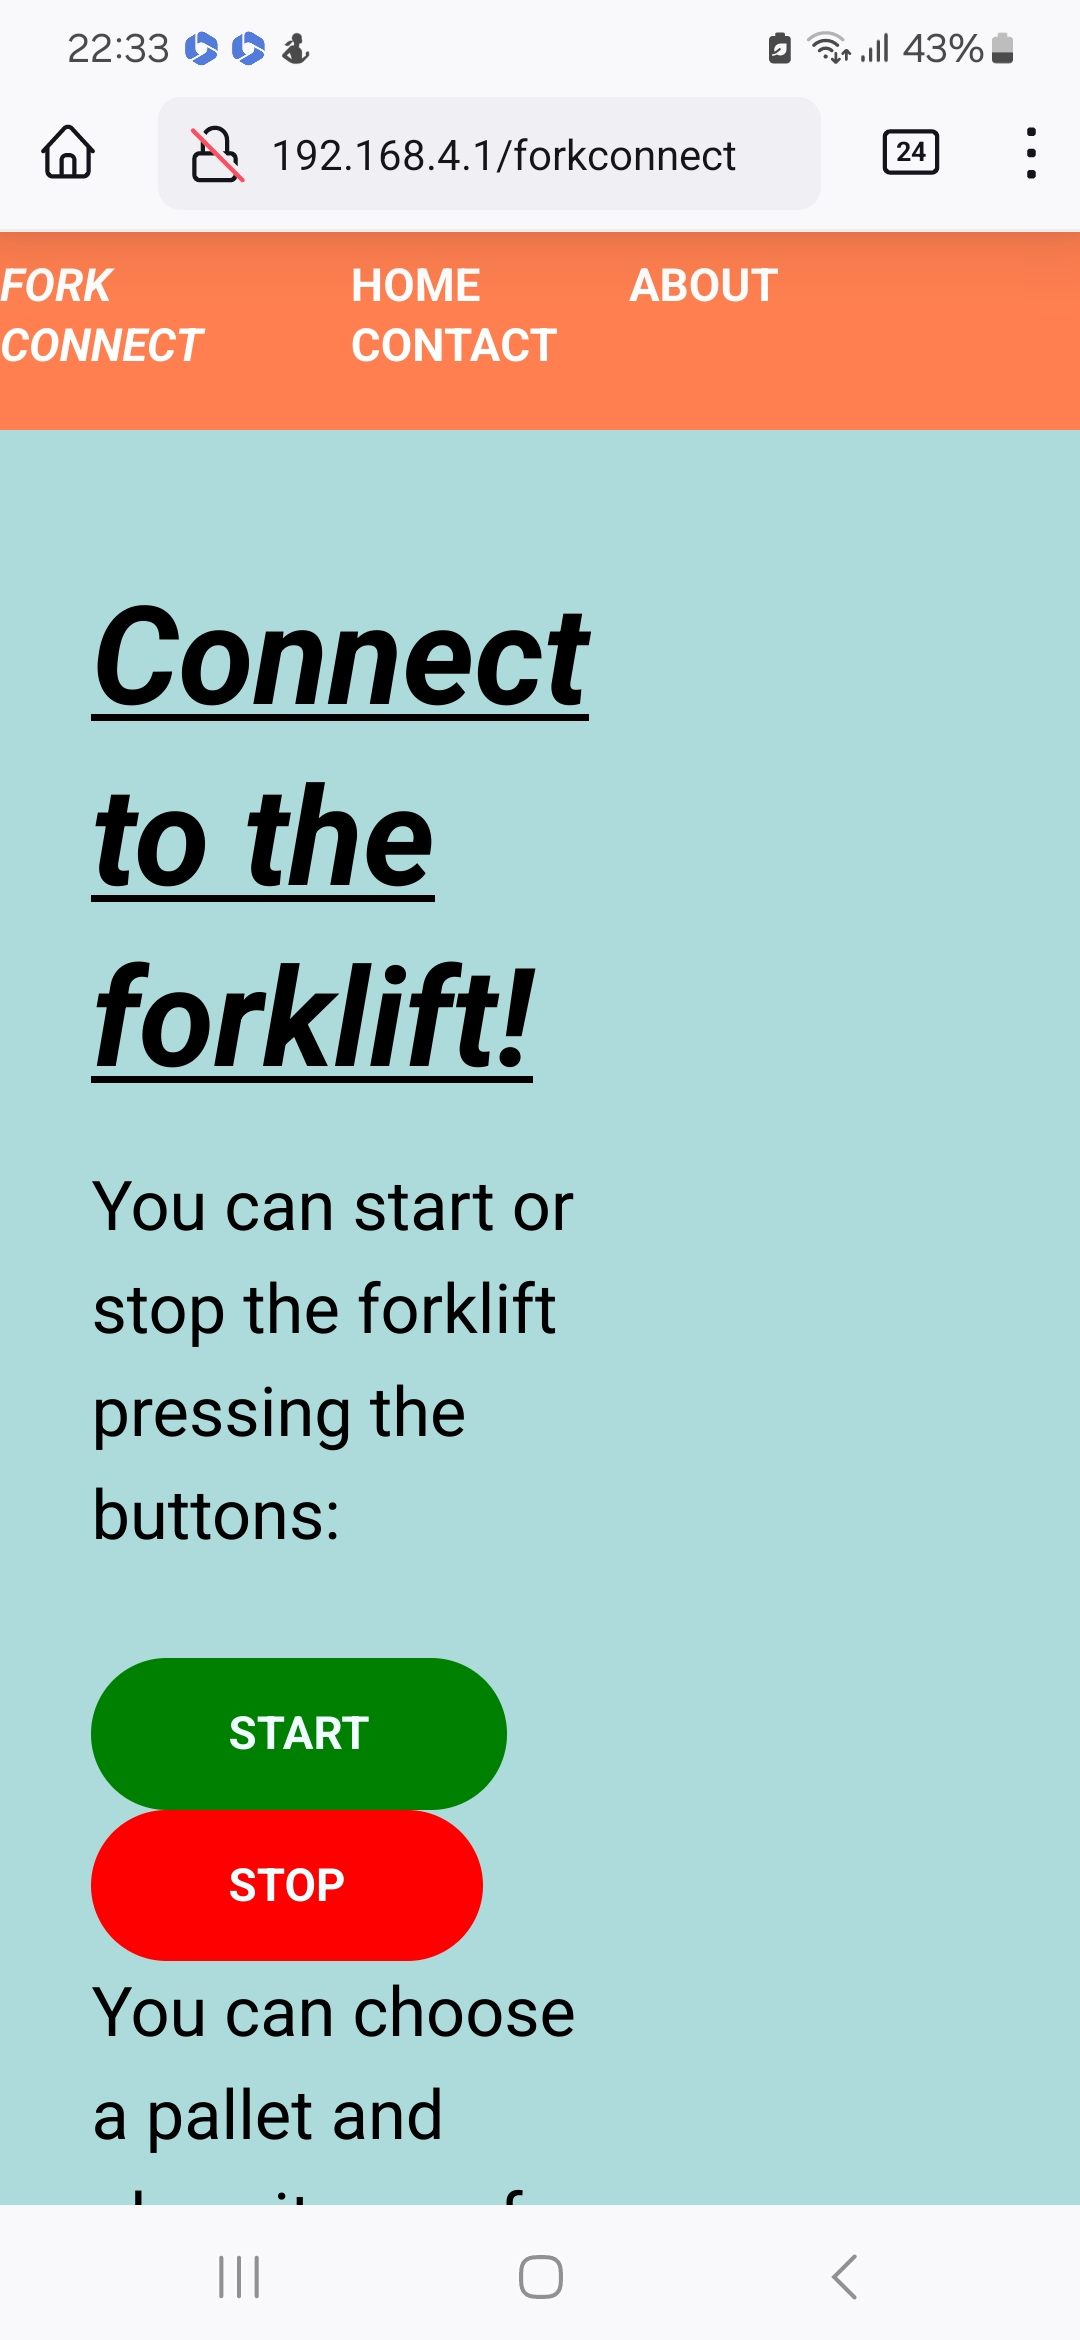
\includegraphics[width=0.24\linewidth]{forkconnect_mobile.jpg}
    \caption{Web frontend on mobile device.}
    
\end{figure} 
\begin{figure}[H]
    \centering
    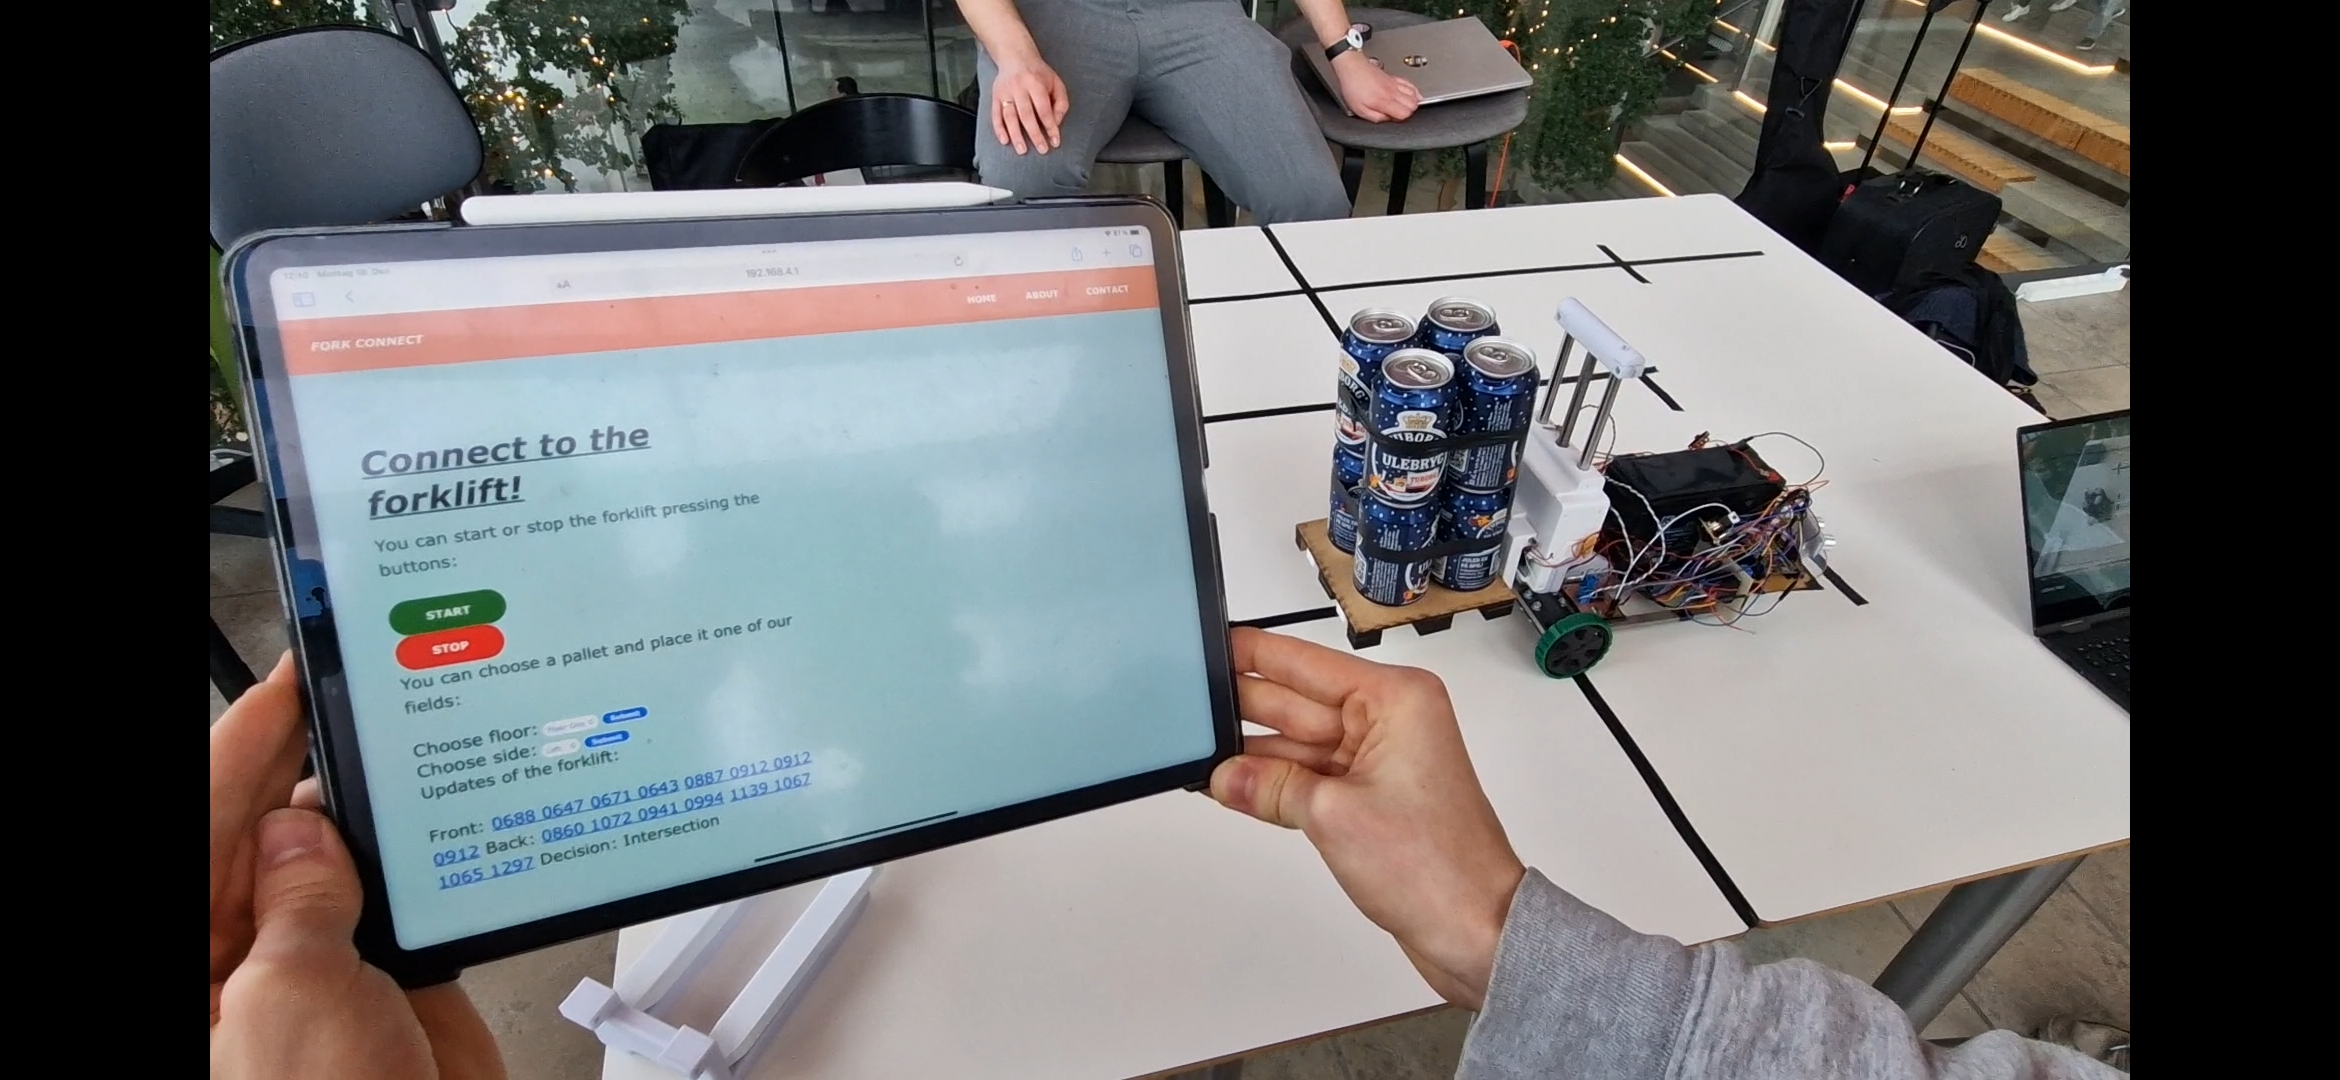
\includegraphics[width=0.75\linewidth]{forkconnect_tekexpo.jpg}
    \caption{Demonstration at TEKExpo. Note the displayed sensor readings and decision.}
\end{figure} 
\subsubsection{The webpage - The frontend}
The webpage is written in html and CSS. The webpage can also be found in the code 
repository (\url{https://github.com/Boti21/SDU-SPRO3-CODE/blob/dev/web_frontend/ForkConnect.html}).
It has a meta statement that causes the web browser to request a new version of the page.
The request will be answered by the http-Server. 

On the website, the user can not only see the sensor readings and decisions that the forklift is doing,
starting and stopping the forklift is also possible with two different buttons: 

\begin{lstlisting}[language=html,caption={The buttons' Code},label={code:webpage}]
    
    <section class="hero">
    <div class="hero-container">
        <div class="column-left">
            <h1>Connect to the forklift!</h1>
            <p> You can start or stop the forklift pressing the buttons:</p>
            <button class="button button1">START </button>
            <button class="button button2">STOP </button>   

\end{lstlisting}
The website also gives the option to send a desired pallet drop off place to the forklift. However,
the backend is not yet working reliably, so in the working forklift prototype the drop of place has to be
entered by the means of code. (There is a bug where the send data includes random characters at the end of the string
send by the connected device).

\end{document}
